\documentclass{template/openetcs_article}
% Use the option "nocc" if the document is not licensed under Creative Commons
%\documentclass[nocc]{template/openetcs_article}
\usepackage{lipsum,url}
\usepackage{supertabular}
\usepackage{multirow}
\usepackage {ulem}
\usepackage{color, colortbl}
\definecolor{gray}{rgb}{0.8,0.8,0.8}
\usepackage[modulo]{lineno}
\usepackage[sharp]{easylist}
\graphicspath{{./template/}{.}{./images/}}
\begin{document}
\frontmatter
\project{openETCS}

%Please do not change anything above this line
%============================


% The document metadata is defined below

%assign a report number here
\reportnum{OETCS/WP3/}

%define your workpackage here
\wp{Work-Package 3: ``Modeling''}

%set a title here
\title{EVC External Interfaces}

%set a subtitle here
\subtitle{openETCS Modeling}

%set the date of the report here
\date{August 2013\\Revised \today}

%define a list of authors and their affiliation here



\author{Baseliyos Jacob}

\affiliation{Deutsche Bahn AG / DB Netz AG\\
  openETCS Project Group \\
  Voelckerstrasse 5\\
  80939 Muenchen, Germany \\
  \\
  eMail: ProjectOffice@openETCS.org \\
  WebSite: www.openETCS.org}


% define the coverart
\coverart[width=350pt]{openETCS_EUPL}

%define the type of report
\reporttype{Description of work}


%\begin{abstract}
%define an abstract here
%  \lipsum[12-13]
%\end{abstract}

%=============================
\maketitle

%Modification history
%if you do not need a modification history table for your document simply comment out the eight lines below
%=============================
\section*{Modification History}
\tablefirsthead{
\hline 
\rowcolor{gray} 
Version & Section & Modification / Description & Author \\\hline}
\begin{supertabular}{| m{1.2cm} | m{1.2cm} | m{6.6cm} | m{4cm} |}
1.0 & & Definition of I\textbackslash O's & B.Jacob \\
 & & & Jan Welvaarts \\\hline
\end{supertabular}


\tableofcontents
%\listoffiguresandtables
\newpage
%=============================

%Uncomment the next line if you need line numbers for tracebility when the document is in review
%\linenumbers
%=============================


% The actual document starts below this line
%=============================

%Start here

 

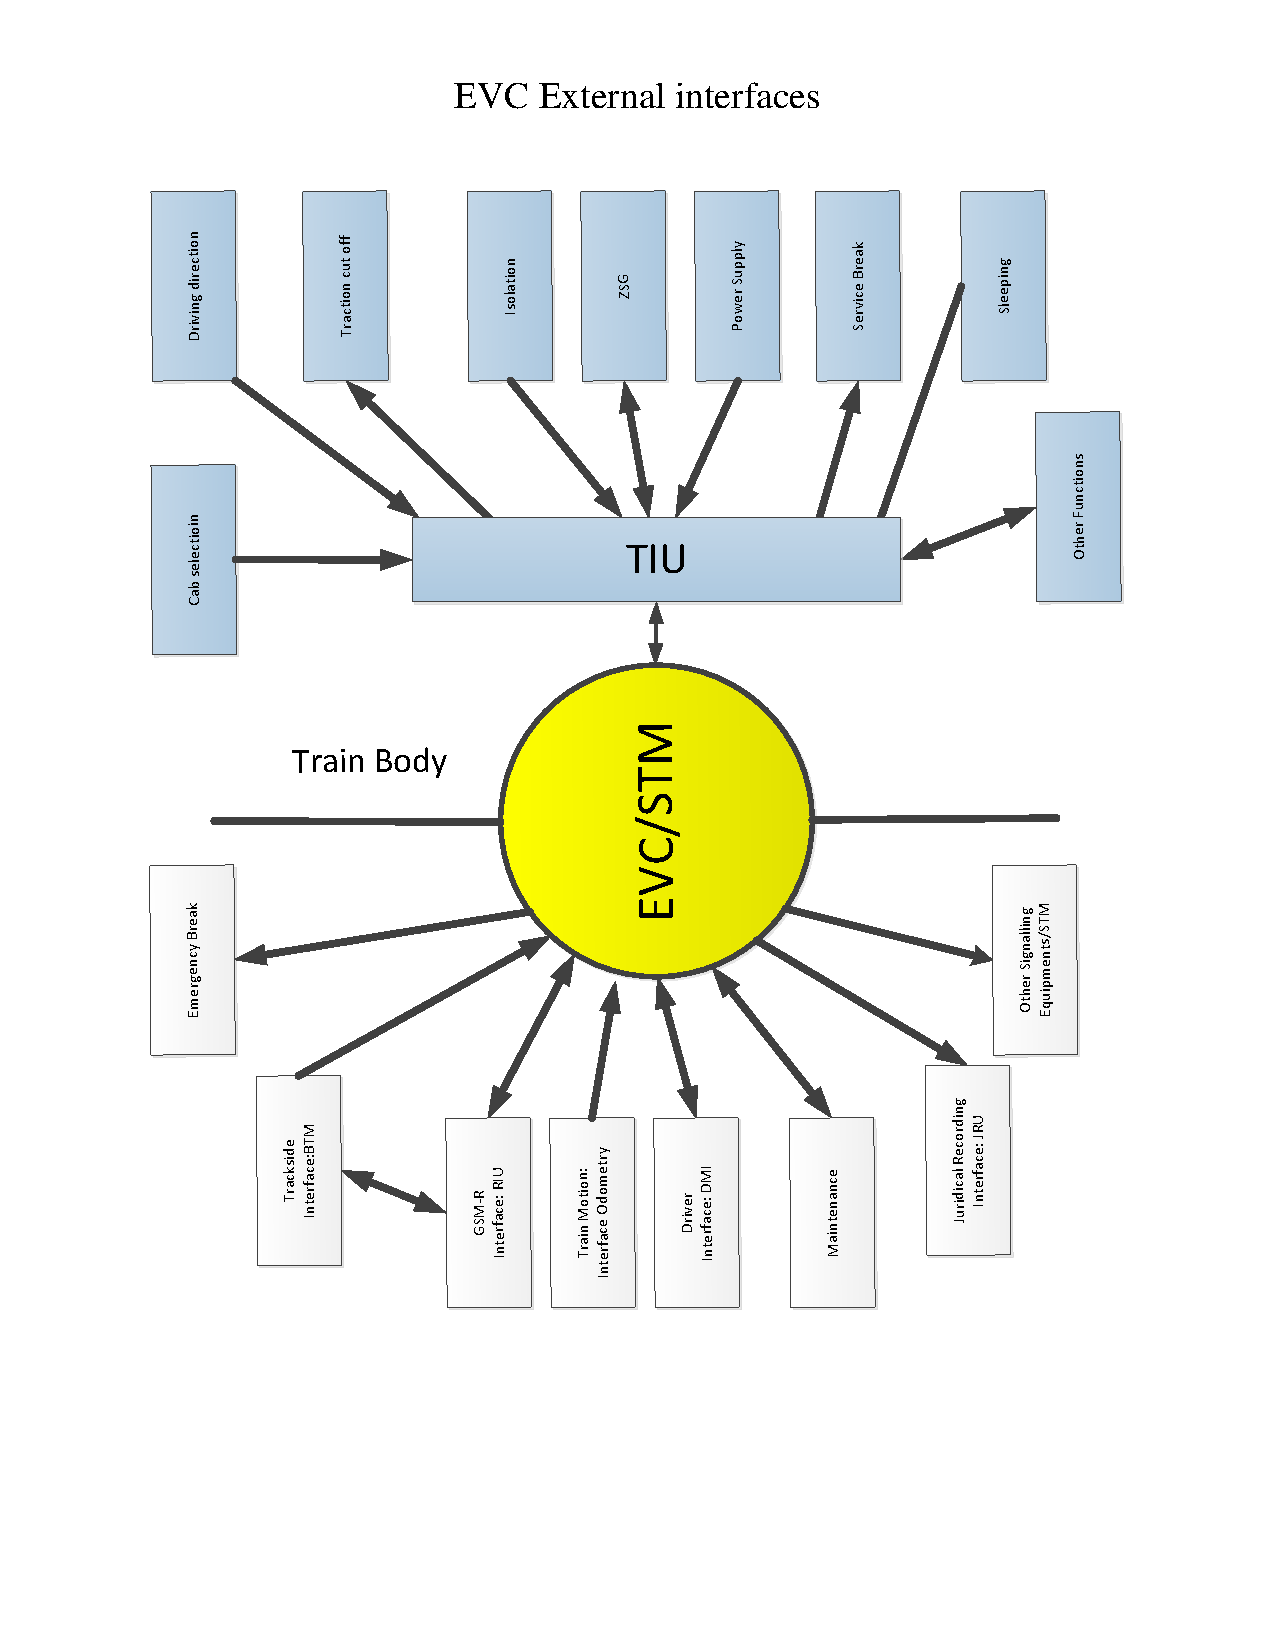
\includegraphics[trim = 20mm 20mm 20mm 10mm, clip, width=15cm]{figs/external_interfaces.pdf}


\begin{tabular}{ l l }
\\
    \textbf{Functional Interface}  & \textbf{Sub-Interface} \\ 
    
    Emergency brake &  EVC EB (BIU) \\ 
   	Air Gap Interface beacons &  EVC (BTM) \\
   	Air Gap Interface loops &  EVC (LTM) \\
   	Air Gap Interface Radio &  EVC (Radio-RBC) \\
    Train motion &  EVC Odometrie (ODO)\\
	Cab selection & Desk state (TIU)\\
	Traction cut-off &  Desk state (TIU)\\
	Driving direction &  Direction controller state (TIU)\\
	Traction cut-off &  Tractioin cut-off (TIU)\\
	Service brake &  Service brake (TIU)*\\
	Sleeping \& Non Leading &  Sleeping (TIU)\\
	Power Supply &  Power supply\\
	Isolation &  EVC Isolation, STM Isolation (TIU)\\
	Driver &  DMI Display (DMI)\\
	Maintenance &  TRU\\
	Other functions &  ZSG, AFB (ICE Germany) (TIU)\\
	Juridical data storage &  (JRU)\\
	Diagnose data storage &  (DRU)\\
	Class B systems &  (STM)\\
    
  \end{tabular}



\section{Installation requirements}

\begin{easylist}
# Interface with the emergency brake
## There shall two independent ERTMS emergency brake commands in the trainset.
## The ERTMS equipment shall control that the command of the emergency brakes is correctly to the train interface.
## Emergency brake command shall be tested during the daily test.


# Cab selection
## Train Body shall provide the cab selection information to the EVC.


# Driving direction

## The Train body shall provide driving direction information to the EVC.
## The ERTMS equipment shall read the driving direction via the Direction Controller State Interface.
## \sout{The ERTMS shall implement a standstill supervision to avoid a movement of the trainset Without direction selected.} This is a specified ETCS function (see roll away protection)


# Interface with traction cut-off

## \sout {ERTMS System shall provide the traction cut-off}  This is a specified ETCS function (see roll away protection)


## Train Body (TIU) shall provide the feedback from the traction cut off system.

## ERTMS function shall command a software traction cut-off via the Traction cut-off Interface of the EVC equipment.

## When ERTMS emergency brakes are applied, when the traction cut off is requested and a low pressure I detected in the main EB pipe, than it is the responsibility of the train driver to cut the traction.


# Interface service brake


## The ERTMS function shall controll the service brake via the Service Brake in interface of the EVC (TIU).

## Monitoring of the Service brake shall be performed by the combination of the Service Brake state and the Odometry declaration (It is an internal function of the EVC).

## In case of simultaneous service brake and emergency brake request, the priority shall be given to the emergency brake.


# Interface with sleeping

## Train Body (TIU) shall provide the sleeping information to the EVC.

## The ERTMS shall detect the request to enter in sleeping mode via the Sleeping interface.

## Train Body (TIU) shall provide the feedback from the traction cut off system.

## ERTMS function shall command a software traction cut-off via the Traction cut-off Interface of the EVC equipment.

## When ERTMS emergency brakes are applied, when the traction cut off is requested and a low pressure I detected in the main EB pipe, than it is the responsibility of the train driver to cut the traction.

# Interface with power supply (not relevant for the SSRS)

## To be able to manage the sleeping mode, the ERTMS equipment shall be allways Powered as soon as the train is powered.

## If longer operation is needed, the driver shall be able to perform a power off/power on sequence to restart the system before exceeding 24 hours.

## Driver shall not use circuit breakers or ERTMS isolation under normal circumstances.

# Interface with ETCS Isolation (not relevant for the SSRS)

## The ERTMS equipment shall be interfaced to an isolation switch. When the equipment is isolated, it shall no more be powered, and no more able to apply the emergency brake.

\end{easylist}



\section{National DMI requirements}
\begin{easylist}
# Interface with the Driver/DMI

## The driver shall interact with the ERTMS equipment via the DMI interface.

## DMI shall display signaling information from ERTMS and STM.

## The DMI shall always display the set speed.

## Only one speed shall be displayed to the driver at any time.

## DMI shall display train information. (braking/traction effort, door status, passenger brake state, SIFA (ICE Germany).

## All train (TCMS) information shall be displayed in the are replacing the ERTMS planning area and in the area below the planning area.

## When the DMI is active the data entry for ETCS and STM shall be performed on DMI.

## Daily test of ETCS and STM shall be launched on the DMI when ETCS is in stand by mode whatever level.

## The DMI shall allow the driver to validate the test result and to display the test with the date of the last test performed.

## If the level 0 is selected, in leaving the Standby mode, a text message shall be displayed on the DMI to the driver to inform him that level 0 is selected. The driver shall acknowledge this message.
\end{easylist}


\section{National odometer (installation) requirements}

\begin{easylist}
# Interface with the train motion

## The ERTMS equipment shall compute the train position and the train speed via the ERTMS Odometry interface. This interface can composed of wheel sensor, radar and accelerometer.

## The wheel diameter to be used by the ERTMS function shall be updated by the maintenance Team by using the DMI interface.


## ERTMS functions and equipments shall have no impact on existing ATP odometry.
\end{easylist}


\section{National requirement?}

\begin{easylist}
# Interface with the JRU (FFFIS Subset 27)

## All juridical information related to the ERTMS equipment shall be recorded and available via the TRU (???) interface.

## \sout{ DMI shall display signaling information from ERTMS and STM.}

## \sout{The DMI shall always display the set speed.}
\end{easylist}

\section{Overview OBU external and EVC external interfaces}



\begin{center}
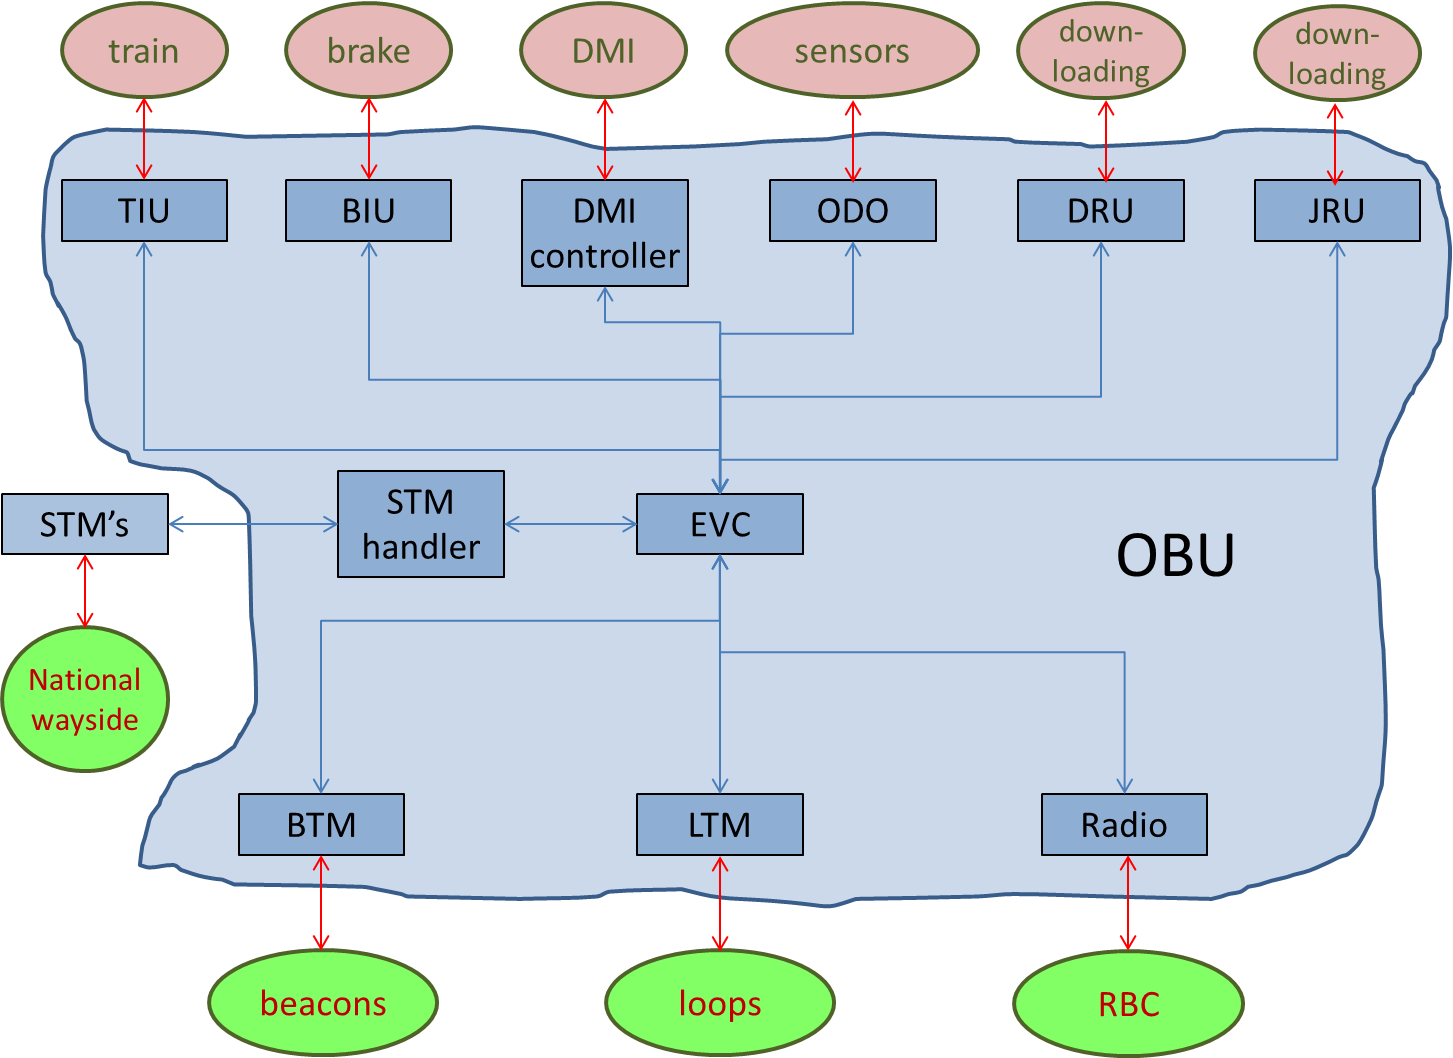
\includegraphics[scale=0.6]{figs/overview_obu}
\end{center}

Today the OBU is the complete ETCS on board installation. The scope of openETCS is limited to the EVC, the part realizing the ETCS functionality.

In the SSRS 
\begin{itemize}
\item the ETCS requirements have to be assigned to the EVC, the different OBU sub functions, the on board installation, the STM's and the wayside systems
\item Requirements assigned to the EVC must be clarified.
\item Functions realizing the requirements have to be described including the input and output data needed ({\textquotedblleft}Data dictionary{\textquotedblright}).

The input and output data can be external for the EVC (to the sub functions described above) or between internal EVC functions 
\item The interfaces between the EVC and the sub functions have to be described including the data format for the information exchanged: {\textquotedblleft}EVC interface specification{\textquotedblright}
\end{itemize}


\section{OBU external interfaces and their specifications:}



\paragraph{TIU/BIU-train}
  \begin{itemize}
  \item Subset 34 (FIS)
  \end{itemize}

\paragraph{DMI controller-DMI}
  \begin{itemize}
  \item ETCS Driver Machine interface ERA\_ERTMS\_015560
  \end{itemize}



\paragraph{ODO-sensors}
\begin{itemize}
\item Not defined
\end{itemize}

\paragraph{DRU-downloading tool}
\begin{itemize}
\item  X
\end{itemize}

\paragraph{JRU-downloading tool}
\begin{itemize}
\item X
\end{itemize}

\paragraph{STM manager-STM{\textquoteright}s}
\begin{itemize}
\item Subset 35
\item Subset 56
\item Subset 57
\item Subset 58
\end{itemize}

\paragraph{BTM-beacons}
\begin{itemize}
\item Subset 36
\end{itemize}

\paragraph{LTM-loops/radio infill}
\begin{itemize}
\item Subset 44
\item Subset 47
\item Subset 48
\end{itemize}

\paragraph{Radio-RBC}
\begin{itemize}
\item subset 37
\end{itemize}


\section{EVC external interfaces and their specifications:}

\paragraph{EVC-TIU/BIU}
\begin{itemize}
\item Information description in subset 34
\end{itemize}

\paragraph{EVC-DMI controller}
\begin{itemize}
\item Information from ETCS Driver Machine interface ERA\_ERTMS\_015560
\end{itemize}
\paragraph{EVC-odometer}
\begin{itemize}
\item 97E2675B
\end{itemize}

\paragraph{EVC-JRU}
\begin{itemize}
\item Subset 27
\end{itemize}

\paragraph{EVC-DRU}
\begin{itemize}
\item Customer specific specifications
\end{itemize}

\paragraph{EVC-STM manager}
\begin{itemize}
\item Information from subset 58
\end{itemize}

\paragraph{EVC-BTM}
\begin{itemize}
\item x
\end{itemize}

\paragraph{EVC-LTM}
\begin{itemize}
\item x
\end{itemize}

\paragraph{EVC-Radio}
\begin{itemize}
\item x
\end{itemize}



Further data descriptions can be derived from:

\begin{itemize}
\item subset 26, chapter 7,
\item {\dots}
\end{itemize}

\section[EVC internal interfaces]{EVC internal interfaces}

\bigskip

The EVC internal interface descriptions will arise from the description of the functions and the information exchanged between them.



Therefore the SSRS will include:

\begin{itemize}
\item Requirements, traceable to the ERA specifications, clarified and assigned to EVC and/or sub functions
\item Description of the EVC functions
\item Internal and external EVC interfaces: the {\textquotedblleft}Data dictionary{\textquotedblright}, and thus the internal EVC architecture.
\end{itemize}


Impression of the EVC internal architecture:

\begin{center}
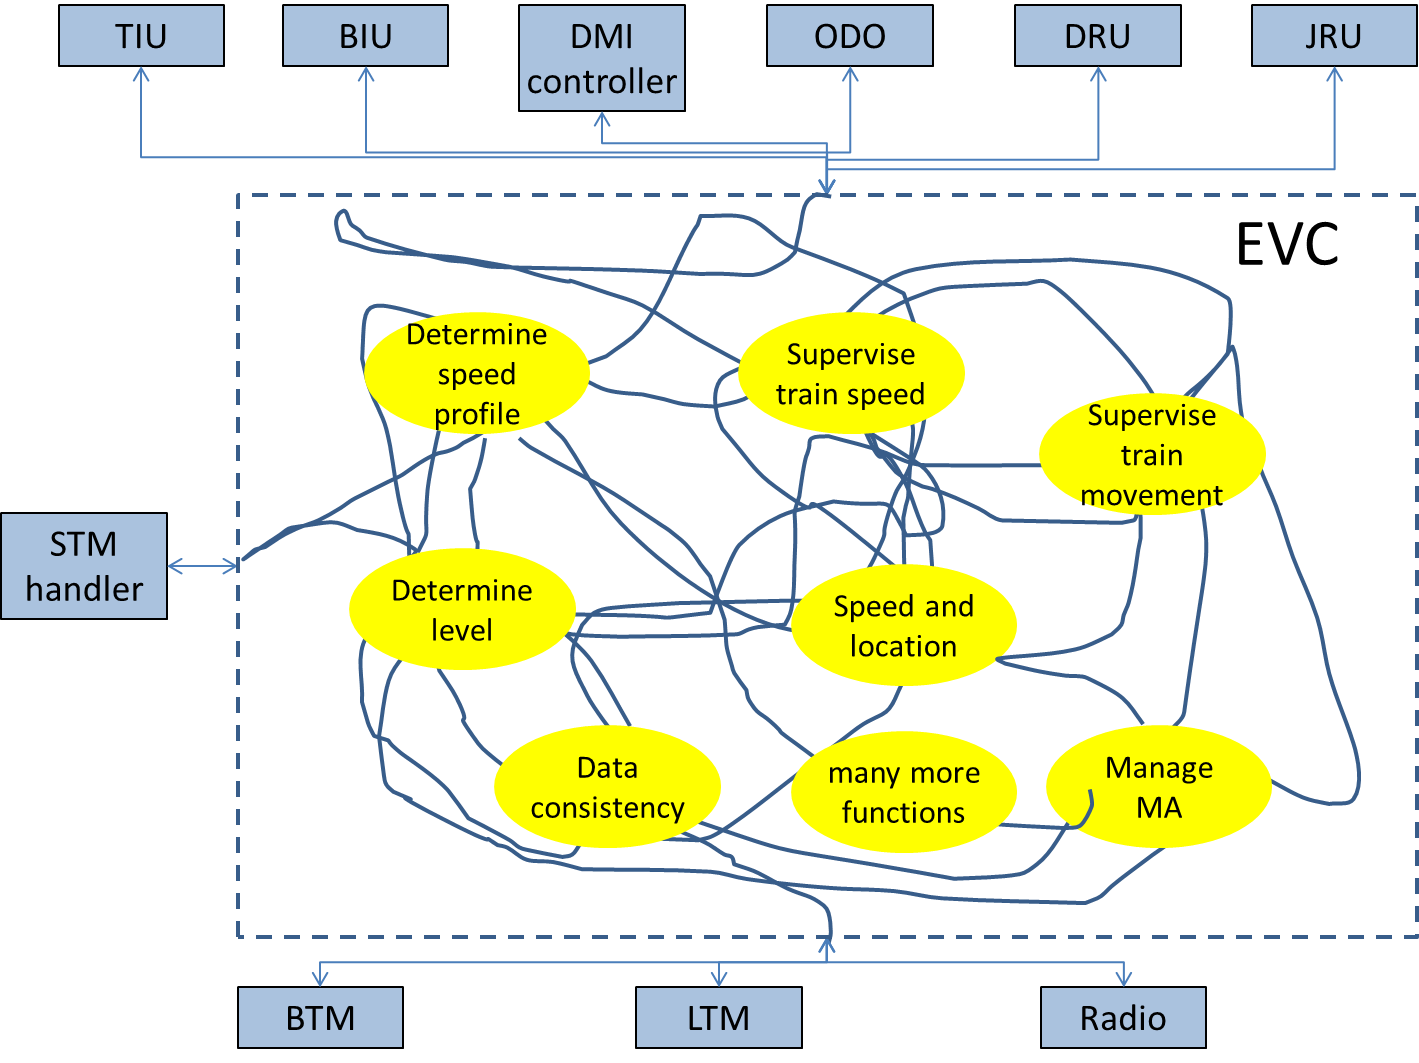
\includegraphics[scale=0.6]{figs/impression}

\end{center}

\end{document}
